\documentclass[12pt]{article}

% --- Packages ---
\usepackage[margin=1in]{geometry} % Sets standard 1-inch margins
\usepackage{amsmath, amssymb}     % Standard math packages
\usepackage{graphicx}             % Required for inserting images
\usepackage{float}                % Allows precise image placement using [H]
\usepackage{booktabs}             % For professional-looking tables
\usepackage{hyperref}             % Makes references and citations clickable
\usepackage{setspace}             % Allows line spacing adjustments
\usepackage{caption}              % Customizing captions for figures/tables

% --- Setup hyperref ---
\hypersetup{
    colorlinks=true,
    linkcolor=blue,
    filecolor=magenta,      
    urlcolor=cyan,
    citecolor=blue,
}

% --- Title Information ---
\title{\textbf{The Cost of Transit Construction}}
\author{
    \vspace{0.3cm}
    \textit{Stats 423: Applied Linear Regression}
}
\date{\today}

\begin{document}

\maketitle

\begin{table}[h]
\centering
\begin{tabular}{p{0.3\linewidth} p{0.65\linewidth}}
\textbf{Name} & \textbf{Contribution} \\[0.5em]

Alison Tan & Model Building and Diagnostics \\[0em]

Katie Gower & Introduction, Data Description \\[0em]

Viki Hristova & Abstract, Conclusion \\[0em]


\end{tabular}
\end{table}


\begin{abstract}
\noindent Increasing urban populations are driving the need for accessible public transportation. However, large scale construction projects often require substantial investments. The Transit Costs Project dataset on transit costs compiles information on transit projects across differing timelines, project scales, and locations in hope of understanding transit project cost variance. 

Our research questions focus on what characteristics of a project drive cost and in what regions projects are more expensive in both cost per kilometer and total real cost, which are in US dollars adjusted for 2023 inflation. To further analyze factors that could explain project costs, we joined data from the World Bank on urban population percentage and GDP. We built simple multiple linear regression models for our two response variables, overall real cost and cost per kilometer, through both direction stepwise model selection, accounting for correlation between attributes, and focusing on adjusted R squared values. 

From our models, we concluded that the main factors influencing the cost of transit projects and length and stations, which are highly correlated, as well as the duration of a project in years, the GDP of the country where a project was constructed, and the continent where the project is located. We also found that projects in Africa were associated with the highest costs and projects in Europe and Asia had the lowest costs.
\end{abstract}

\onehalfspacing % 1.5 spacing makes it easier for grading

% -------------------------------------------------------------------
\section{Introduction}
% -------------------------------------------------------------------

Public transit works to move people where they live, work, and play. In recent years, people have been advocating for an increase in transit access to reduce car dependence. With demand growing, it is necessary to increase transit infrastructure. However, cost of construction and time to complete projects are barriers in the public transit transition.

The Transit Costs dataset was created with hopes of understanding what affects the cost of public transit construction projects. It covers many types of transit projects such as railroad,  tunnel, elevated, lightrail, and subway and sixty countries across all continents except Antarctica. The observations are most concentrated in the past three decades.

\subsection{Research Questions}
\begin{enumerate}
    \itemsep-0.5em 
    \item What characteristics of projects drive cost per km? 
    \item What regions are projects more expensive in by kilometer?
    \item What attributes create a more expensive project overall?
    \item What regions are projects more expensive in overall?
\end{enumerate}

% -------------------------------------------------------------------
\section{Data Description and Exploratory Data Analysis (EDA)}
% -------------------------------------------------------------------

\subsection{Variables}

Response variables:
\begin{itemize}
    \itemsep-0.5em 
    \item Cost per kilometer in millions of US dollars (2023 dollars)
    \item Total real cost in millions US dollars (2023 dollars)
\end{itemize}
Predictors:
\begin{itemize}
    \itemsep-0.5em 
    \item Year: Midpoint of project completion (Numeric)
    \item Stations: Number of stations (Numeric)
    \item Length: Length of line in kilometers (Numeric)
    \item RR: Regional Rail or not (Logical)
    \item Country: Country Project is in (Categorical)
    \item Elevated: Length in kilometer of elevated line (Numeric)
    \item TunnelPer: Percentage of line that is tunnel (Numeric)
    \item AtGrade: Length of line at grade/ground level (Numeric)
    \item Start Year (Numeric)
    \item End Year (Numeric)
    \item GDP: Real GDP for country and year (Numeric)
\end{itemize}
Variables created:
\begin{itemize}
    \itemsep-0.5em 
    \item Years: End Year - Start Year (Numeric)
    \item Continent: Continent the construction took place in (Categorical)
\end{itemize}

\subsection{Exploratory Analysis}

The transit costs dataset includes monetary values are in millions of real US dollars. GDP was measured in real US dollars. Measures of length were in kilometers. Due to some attributes being set as character despite being numbers, we casted some columns as numeric or factor. We were interested in continent and years to complete which were not included in the original data set, but were easily created based on existing information. 

There were missing values in the data present, most notibably for atgrade with 404 NAs and atgrade with 392. We chose to not use these values as predictors to keep more viable observations rather than lose around 400. Real cost's NA values were accounted for by multiplying real cost/kilometer and length in kilometers, which also matched well to existing values. To get the project year length for all values, we added values for start year and end year by adding or subtracting half of average years to complete for the continent of that observation. If both start and end year were missing, half the average project year length by continent was added or subtracted to the year, the midpoint of project completion. Asia and Africa originally had substaintially more missing values for years than other continents, but after imputation there were none.

GDP data was pulled from World Bank. The original format was rows corresponding to countries and columns corresponding to years. Data transformation was done to assign each row of the transit costs dataset a GDP value for the country of the project in the project’s midpoint year. Urban population was also from World Bank and had a similar format, although we hypothesized it could be a good predictor it was not in any final models

\begin{figure}[H]
    \centering
    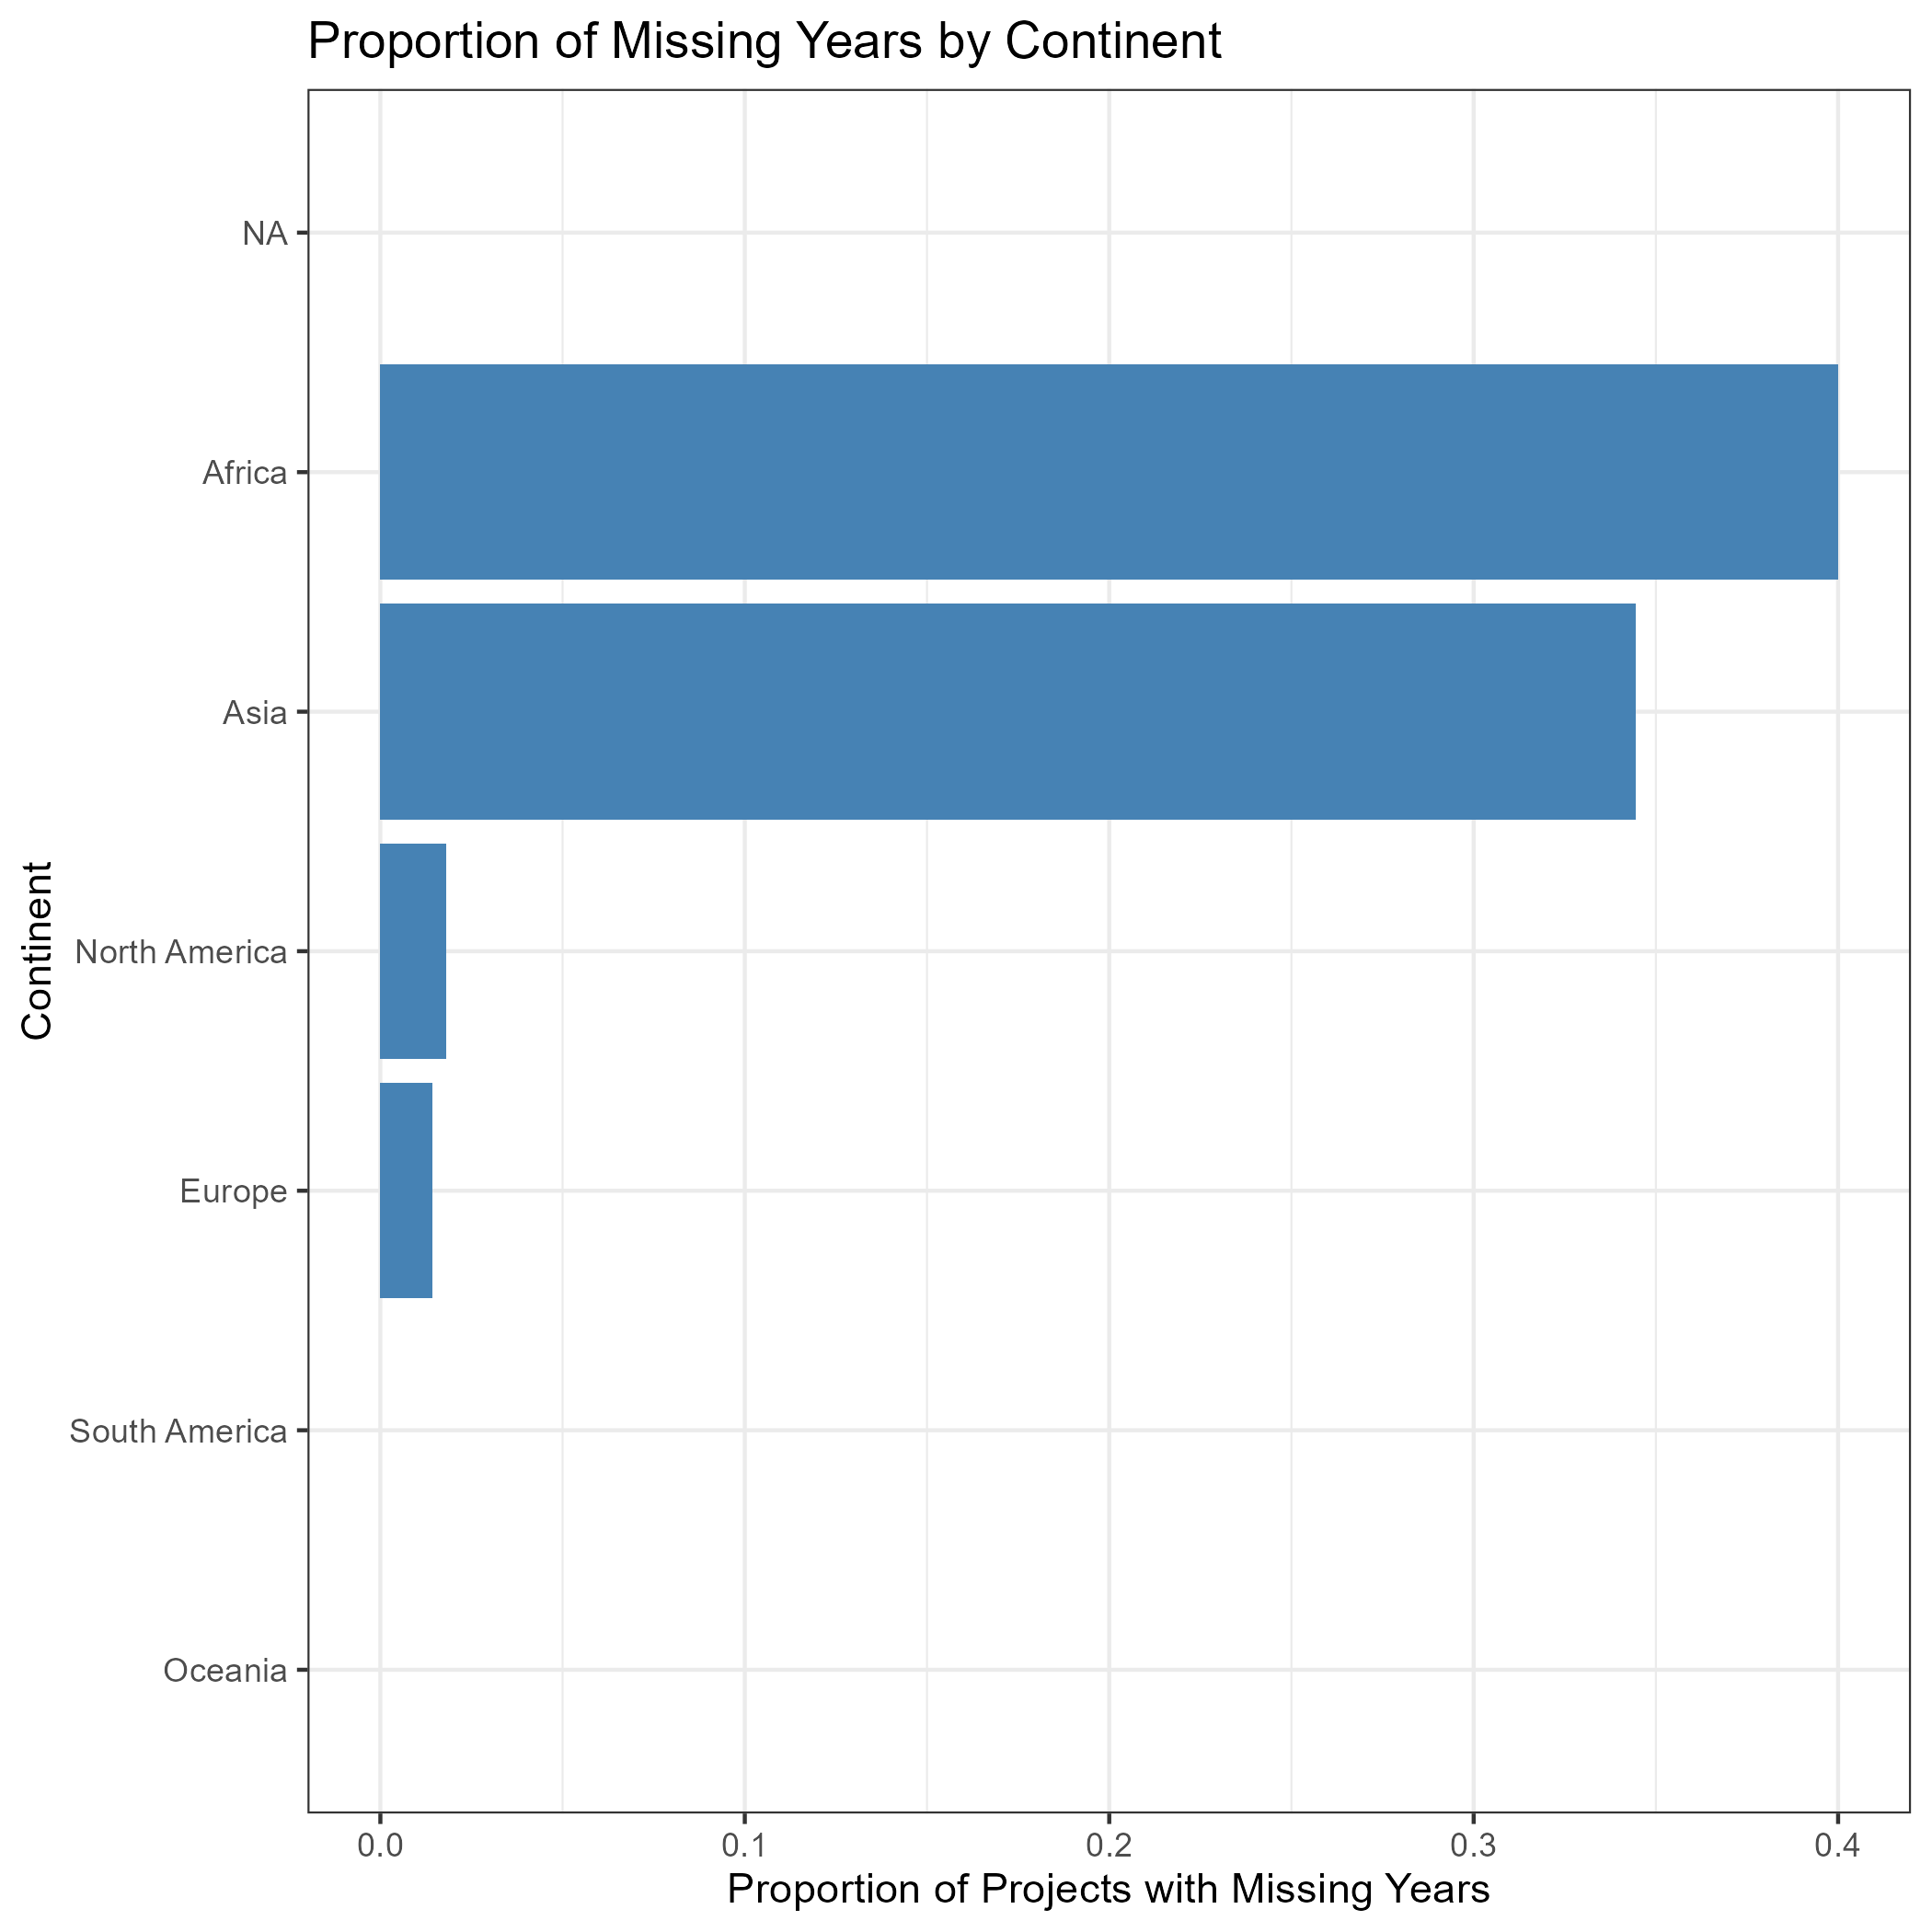
\includegraphics[width=0.3\linewidth]{plots/missing-years-by-continent.png}
    \caption{Proportion of Missing Years by Continent}
    \label{fig:missyears}
\end{figure}

% -------------------------------------------------------------------
\section{Methodology and Model Building}
% -------------------------------------------------------------------
\subsection{Proposed First Model}
$$log(CostPerKm) = -4.83 + 0.027Years +0.005StartYear + 0.0055TunnelPer - 1.35ContinentAsia $$
$$-1.24ContinentEurope-0.81ContinentOceania -0.94ContinentSouthAmerica $$
$$ - 0.81ContinentNorthAmerica -0.19PPPRate +\epsilon_i$$
where $\epsilon_i \overset{iid}{\sim} \mathcal{N}(0, \sigma^2)$.

\subsection{Proposed Second Model}
    $$Total Cost = 57.91 + 0.157*TunnelPer + 0.488 *Years + 1.223*Length + -3.1e-13*GDP $$
    $$-31.23*ContinentAsia -45.75*ContinentEurope -24.36*ContinentNorthAmerica - $$
   $$ 23.60*ContinentOceania-24.18*ContinentSouthAmerica + \epsilon_i$$


where $\epsilon_i \overset{iid}{\sim} \mathcal{N}(0, \sigma^2)$.

\subsection{First Model Selection and Summary}

\vspace{12pt}
\begin{tabular}{lrrrr}
\hline
\textbf{Predictor} & \textbf{Estimate} & \textbf{Std. Error} & \textbf{t-value} & \textbf{Pr($>|t|$)} \\
\hline
(Intercept) & -4.8386861 & 4.0279853 & -1.201 & 0.229993 \\
Years & 0.0274532 & 0.0060991 & 4.501 & 7.73e-06 \\
Start.year & 0.0054683 & 0.0020058 & 2.726 & 0.006542 \\
TunnelPer & 0.0055893 & 0.0004717 & 11.848 & $< 2e^{-16}$ \\
ContinentAsia & -1.3481124 & 0.2395711 & -5.627 & 2.51e-08 \\
ContinentEurope & -1.2433227 & 0.2384818 & -5.213 & 2.34e-07 \\
ContinentNorth America & -0.8059310 & 0.2467630 & -3.266 & 0.001136 \\
ContinentOceania & -1.0861986 & 0.3600030 & -3.017 & 0.002630 \\
ContinentSouth America & -0.9436826 & 0.2721792 & -3.467 & 0.000553 \\
PPP.rate & -0.1978282 & 0.0262669 & -7.531 & 1.32e-13 \\
\hline
\end{tabular}

\vspace{12pt}
A log transformation created a more normal distribution of cost/km.

The initial model started with all variables: log\_cost ~ Years + Start.year + Length + Stations + 
    TunnelPer + PPP.rate + gdp + urban\_pop

Bidirection stepwise selection was performed while looking at AIC. The urban population variable was the only variable removed.

\begin{figure}[H]
    \centering
    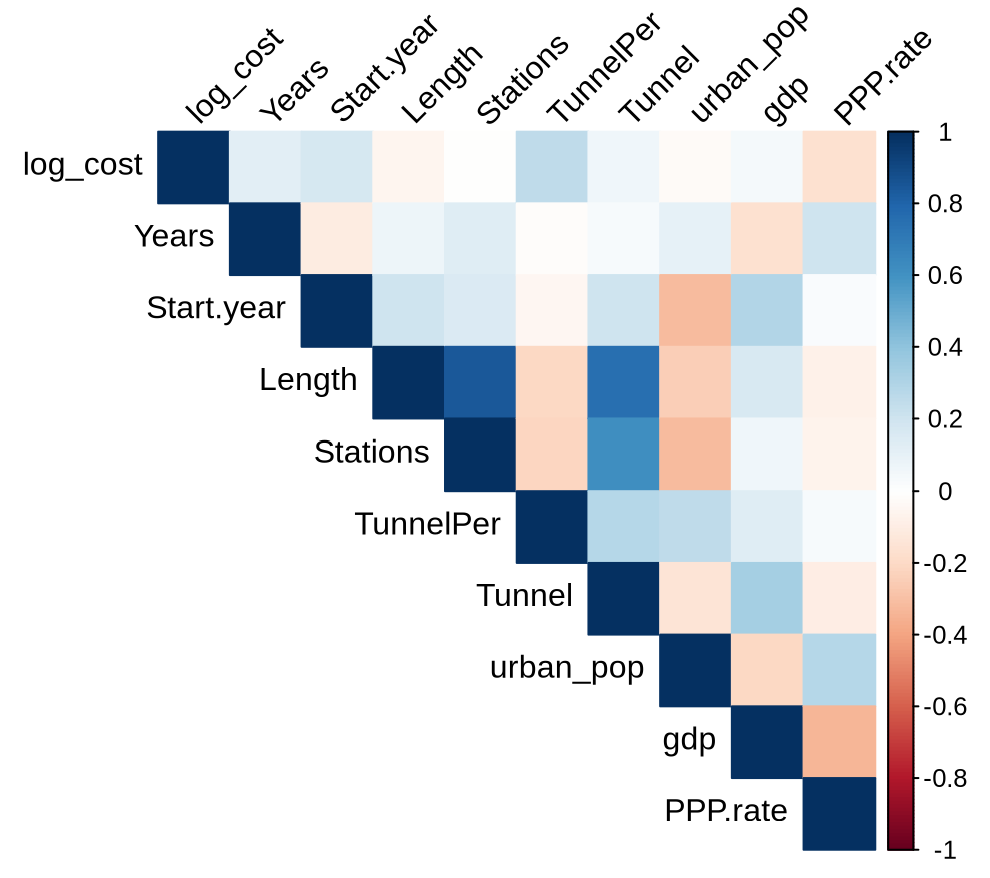
\includegraphics[width=0.3\linewidth]{plots/Correlation plot (log cost km).png}
    \caption{Correlation of Possible Log Cost/km Variables}
    \label{fig:missyears}
\end{figure}

GDP and PPP rate measure similar things and are slightly correlated. We removed the one that resulted in the smaller R squared, which was GDP. Finally, we added continents as a categorical predictor to the model. After doing so, length became insignificant (high p-value) so we removed it, giving us the final model.



\subsection{Second Model Selection and Summary}

\vspace{12pt}

\begin{tabular}{lrrrr}
\hline
\textbf{Predictor} & \textbf{Estimate} & \textbf{Std. Error} & \textbf{t-value} & \textbf{Pr($>|t|$)} \\
\hline
\label{tab:results}
(Intercept) & 5.791e+01 & 8.365e+00 & 6.924 & 8.86e-12 \\
Years & 4.884e-01 & 2.064e-01 & 2.367 & 0.018175 \\
ContinentAsia & -3.123e+01 & 8.231e+00 & -3.794 & 0.000159 \\
ContinentEurope & -4.575e+01 & 8.247e+00 & -5.547 & 3.91e-08 \\
ContinentNorth America & -2.436e+01 & 8.528e+00 & -2.856 & 0.004396 \\
ContinentOceania & -2.360e+01 & 1.243e+01 & -1.899 & 0.057911 \\
ContinentSouth America & -2.418e+01 & 9.391e+00 & -2.575 & 0.010205 \\
gdp & -3.188e-13 & 1.044e-13 & -3.054 & 0.002329 \\
Length & 1.223e+00 & 3.262e-02 & 37.474 & $< 2e^{-16}$ \\
TunnelPer & 1.571e-01 & 1.702e-02 & 9.230 & $< 2e^{-16}$ \\
\hline
\end{tabular}

\vspace{10pt}
With the difficulties of predicting cost per kilometer, we pivoted our focus to total cost. We started with an initial model that did not use continents. When looking at the initial model (real\_cost $\sim$ Stations + gdp + RR. + TunnelPer) AIC, BIC, R squared values and residual plots, a square root transformation was tothe best option to increase Adjusted R Squared without sacrificing model assumptions.
	
Once we settled on a square root transformation, we added all the possible predictors in (excluding continents). We removed RR after using bidirectional stepwise selection and removed urban pop and tunnel percentage because they had high p-values, therefore making them insignificant predictors. Stations was also removed, because it’s highly correlated with length, which resulted in the best adjusted R squared. 

Our final model, once continents were added, had an Adjusted R Squared of 0.7008. We started with 1007 and our final model had 824 degrees of freedom due to NAs that could not be removed.

We were also interested in analyzing what impacts project year length and unfinished projects, but the imputation of missing values would have required making unreasonable assumption. We chose not to study either response variable and focus on cost instead.


% -------------------------------------------------------------------
\section{Diagnostics}
% -------------------------------------------------------------------

\subsection{First Model Diagnostics}

To assess how reliable our model was and if the assumptions of the model were satisfied, we looked at our residual plots, the QQ plot along with a Kolmogorov-Smirnov test, GVIF—not VIF since Continents was factored—and conducted Durbin-Watson and Moran’s I tests for spatial and auto correlation. 

The highest GVIF value was 1.49, so none were over 2 and we had no concern about multicollinearity. 

\begin{figure}[H]
    \centering
    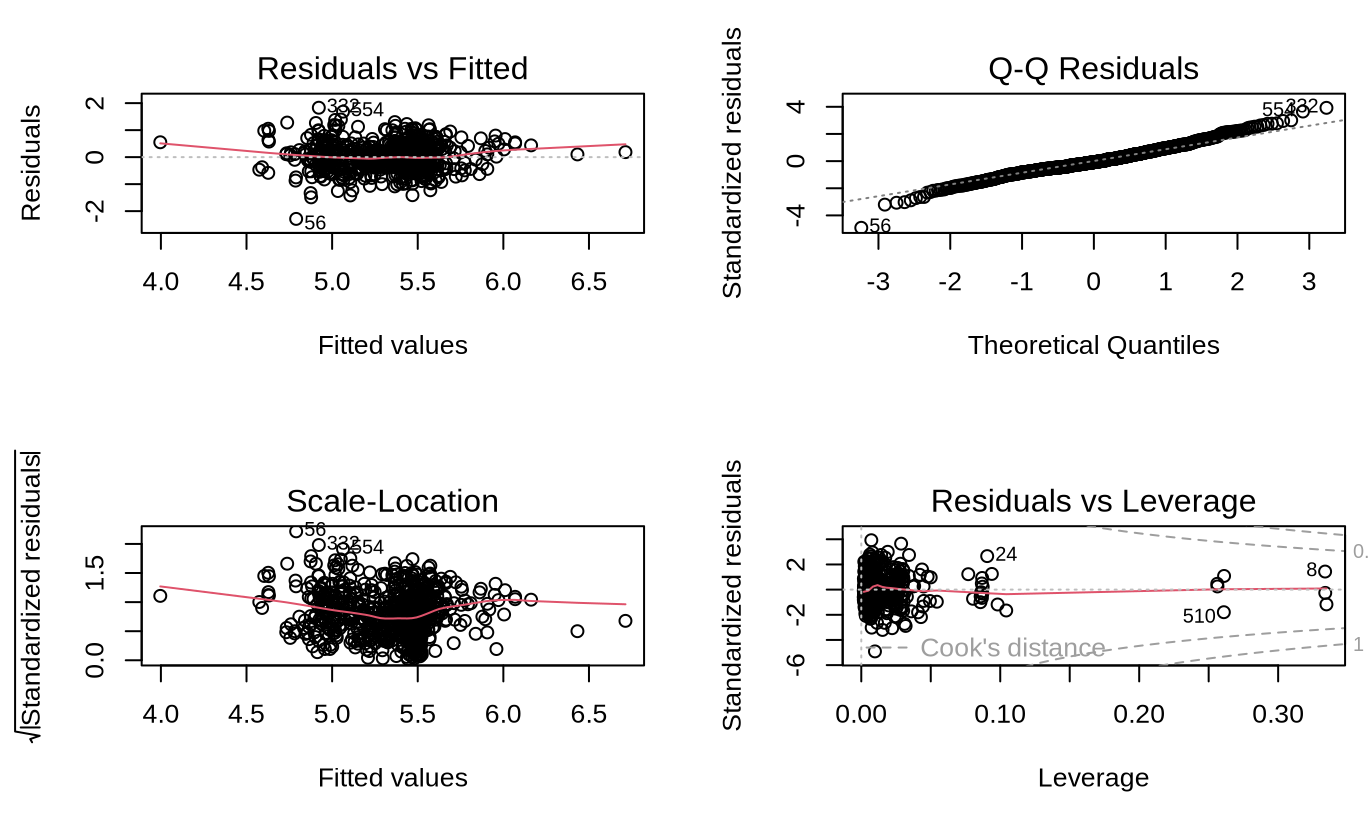
\includegraphics[width=0.55\linewidth]{plots/Final cost km model residuals.png}
    \caption{Cost per kilometer Diagnostic Plots}
    \label{fig:missyears}
\end{figure}

Looking at the residual plots, we see that most of our model assumptions are satisfied. There seems to be an even scattering of residuals around 0, with no evidence of heteroskedasticity, and the points on the QQ plot follow the linear line well, indicating normality of residuals. 

Finally looking at autocorrelation and spatial correlation to attempt to satisfy our independence assumption, we conducted a Durbin-Watson  and Moran’s I test. The Durnin-Watson test indicated that there was evidence of autocorrelation, and the Moran’s I test indicated that there was no evidence of spatial correlation. We attempted various transformations, but these were unsuccessful in addressing autocorrelation. So, our independence assumption is not satisfied. 

This mild violation of our regression assumptions may raise problems and reduce the accuracy of our model. It is likely that different transformations we did not consider, or some time-related structure that we did not consider in our model could further improve the model and satisfy all of our model assumptions. 


\subsection{Second Model Diagnostics}

We approached model diagnostics for this model in the same manner as we did model 1. To assess how reliable our model was and if the assumptions of the model were satisfied, we looked at our residual plots, the QQ plot along with a Kolmogorov-Smirnov test, GVIF—not VIF since Continents was factored—and conducted Durbin-Watson and Moran’s I tests for spatial and auto correlation. The highest GVIF value was 1.86, so none were over 2 and we had no concern about multicollinearity. 

\begin{figure}[H]
    \centering
    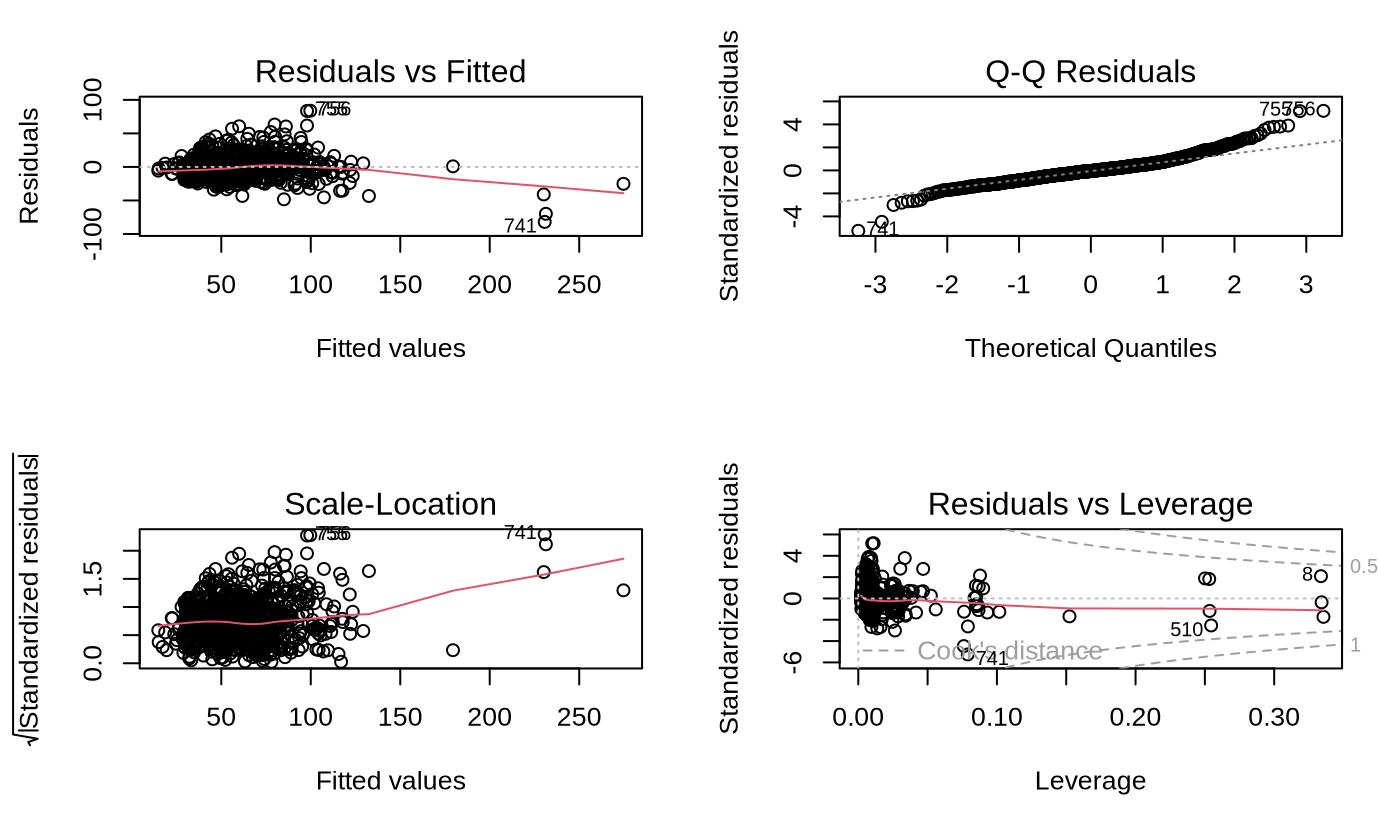
\includegraphics[width=0.55\linewidth]{plots/Final real cost residuals.png}
    \caption{Total Cost Diagnostic Plots}
    \label{fig:missyears}
\end{figure}

Looking at the residual plots, we see some green and red flags. The residuals versus leverage plot shows us that there aren’t any values with a Cook’s distance above 0.5, meaning there aren’t any highly influential points dominating the model. The QQ plot shows some deviations from normality in the tails and our Kolmogorov-Smirnov test failed, but since the sample size is so large, these are unlikely to be problematic. We can see that without the higher fitted values, our residuals are approximately centered around 0 and there is relatively constant variance. However, after observing these outliers and researching these projects, these are valid data points and cannot be removed from our dataset.

Finally, we looked at autocorrelation and spatial correlation to attempt to satisfy our independence assumption. We conducted a Durbin-Watson and Moran’s I test. Both of these resulted in small p-values and rejected their null hypotheses, indicating that there was evidence of spatial and auto correlation. Throughout the project, we attempted various transformations, and pulled in regional data such as gdp and urban population, to account for these. They were unsuccessful.

These mild violations of our regression assumptions may raise problems and reduce the accuracy of our model. It is likely that different transformations we did not consider, the addition of geographic or regional predictors, and other predictors could further improve the model and better satisfy the assumption. 


% -------------------------------------------------------------------
\section{Discussion and Conclusion}
% -------------------------------------------------------------------

In this report, we analyzed attributes' influence on transit construction projects. Overall, we found that location does make an impact, with Asia and Europe having cheaper construction costs. The continents in order from the most to least expensive projects on average are Africa, Oceania, South America, North America, Asia, and Europe.
 
However, with an adjusted R squared value of 0.2252, there is a large amount of unexplained variance in our first model predicting the log cost per kilometer in millions of 2023 USD. Our second model, which predicts the square root of real cost in 2023 USD, included the percent of a transit project that is tunnel as a predictor with a coeffiecient of 0.1571. This means that if a project was 100\% tunnel, the model would estimate the square root of the cost to be 15.71 million dollars more on average than an equivalent project that was not tunnel at all. GDP’s coefficient was -3.2e-13, meaning for each dollar of GDP for the country and midpoint year of the project, the square root of the total cost in millions of dollars goes down by a small amount. Still, GDPs of different countries can be trillions of dollars apart from each other, increasing the influence of small changes. Project length’s coefficient was 1.22. Therefore, for each kilometer of extra length, the model’s estimate increases by at least 1.48 million.
 
Overall, transit project costs can be impacted by a variety of factors each with varying magnitudes of influence. Length and location are two main factors, though. Another likely influential factor is the type of transit project such as lightrail, train, or subway. However, this data does not include this as an attribute. In addition, variation in transit construction cost may be impacted by supply chain issues, especially if the project was constructed during COVID lockdown which can be analyzed in the future.


% -------------------------------------------------------------------
\section*{References}
% -------------------------------------------------------------------

Levy, A., et al. Construction Costs of Urban Rail Projects Worldwide. New York University, 15 Jan. 2025, doi:10.58153/9wnjp-kez15.
\vspace{6pt}
“Why Do Domestic Subway and Light Rail Projects Cost More and Take Longer to Construct than Similar Projects in Italy, Sweden, Turkey, Korea, Chile, and Spain?” Transit Costs Project, 6 Mar. 2026, transitcosts.com/.
\vspace{6pt}
“GDP (Current US\$).” World Bank Open Data, data.worldbank.org/indicator/NY.GDP.MKTP.CD?most\_recent\_year\_desc=true.
\vspace{6pt}
Brazil, Noli. “Lab 7: Spatial Autocorrelation.” CRD 230: Spatial Methods in Community Research, 22 Feb. 2023, https://crd230.github.io/lab7.htmlx`x
\vspace{6pt}
“Urban Population (\% of Total Population).” World Bank Open Data, data.worldbank.org/indicator/SP.URB.TOTL.IN.ZS.

% -------------------------------------------------------------------
\newpage
\appendix
\section{Appendix: R Code}
% -------------------------------------------------------------------
Paste your analysis code here. If you prefer, you can use the \texttt{verbatim} environment to format it as raw text:

\begin{verbatim}
# Example R Code
model <- lm(Y ~ X1 + X2, data = mydata)
summary(model)
plot(model)
\end{verbatim}

\end{document}